
\chapter{Analyse et spécification des besoins}
\label{chap:deuxiemechapitre}

\section{Introduction}

\raggedbottom

\section{Spécification des besoins}

\vspace{5mm}
\subsection{Identification des acteurs}
\vspace{5mm}

\vspace{3mm}

\subsection{Besoins fonctionnels}
\vspace{5mm}
Les besoins fonctionnels représentent les fonctionnalités ou les actions spécifiques que le système doit
effectuer. Ils décrivent les actions que les utilisateurs attendent du système et les résultats attendus de
ces actions.
\par
\vspace{2mm}
Dans cette section, nous expliquerons les fonctionnalités générales de notre système associés à chaque acteur :
\vspace{8mm}

\begin{enumerate}
  \item \textbf{Administrateur: } En tant que responsable de l'application, l'administrateur doit avoir accès à des fonctionnalités de gestion avancées pour assurer le bon fonctionnement de la plateforme. Les besoins fonctionnels de l'administrateur incluent :
  \vspace{4mm}
        \begin{itemize}[label=$\bullet$]
          \item Gestion des Utilisateurs: L'administrateur doit pouvoir créer, modifier et supprimer des comptes utilisateur, ainsi que gérer leurs autorisations d'accès.
          \vspace{3mm}
          \item Gestion des Contenus: Capacité à superviser les fichiers téléchargés par les utilisateurs, à modérer le contenu inapproprié et à assurer la conformité aux directives de sécurité.
          \vspace{3mm}
          \item Personnalisation de l'Application: Possibilité de personnaliser l'apparence et les fonctionnalités de l'application en fonction des besoins des utilisateurs.
        \end{itemize}
\vspace{5mm}
  \item \textbf{Utilisateur (avec abonnement gratuit):}Les utilisateurs normaux sont ceux qui utilisent l'application sans abonnement premium. Leurs besoins fonctionnels comprennent les fonctionnalités de base. Parmi ces fonctionnalités, on trouve :
  \vspace{4mm}
        \begin{itemize}[label=$\bullet$]
          \item Calendrier des Événements et Deadlines: Accès à un calendrier intégré pour planifier et suivre les événements académiques et les échéances importantes.
          \vspace{3mm}
          \item Espace de Notes: Possibilité de créer, éditer et organiser des notes pour prendre des informations importantes.
          \vspace{3mm}
          \item  Gestion des Tâches: Fonctionnalité pour créer des tâches, définir des rappels et suivre les progrès des travaux marqués.
          \vspace{3mm}
          \item Gestion des Fichiers: Capacité à télécharger, organiser et partager des fichiers tels que des cours, des photos, des documents etc.

        \end{itemize}
\vspace{5mm}
    \item \textbf{Utilisateur (avec abonnement premium):}Les utilisateurs premium bénéficient d'avantages supplémentaires pour optimiser leur expérience d'apprentissage et maximiser leur efficacité académique. En plus des fonctionnalités offertes aux utilisateurs normaux, les utilisateurs premium ont accès à des outils avancés basés sur l'intelligence artificielle (IA) pour une gestion encore plus optimale de leurs études. Leurs besoins fonctionnels comprennent donc :
    \vspace{4mm}
         \begin{itemize}[label=$\bullet$]
          \item Stockage Supplémentaire: Capacité à stocker un plus grand nombre de fichiers et à bénéficier d'un espace de stockage illimité.
          \vspace{3mm}
          \item Personnalisation Avancée: Possibilité de personnaliser davantage l'apparence et les fonctionnalités de l'application selon leurs préférences individuelles.
          \vspace{3mm}
          \item Classification Automatique des Cours: L'outil IA intégré permet aux utilisateurs premium de classifier automatiquement les cours qu'ils ont téléchargés et de les organiser dans des dossiers spécifiques, simplifiant ainsi la gestion et la navigation des contenus.
          \vspace{3mm}
          \item Recommandation d'Emploi du Temps Personnalisé: Un autre outil IA avancé analyse divers facteurs tels que les horaires d'études, les progrès académiques, les notes, les horaires de révision, etc. Il utilise ces données pour recommander un emploi du temps individuel spécifique à chaque utilisateur, garantissant ainsi une optimisation maximale du temps d'étude et des performances académiques.
          \vspace{3mm}
          \item  Support Prioritaire: Accès à un support client prioritaire pour résoudre rapidement les problèmes et répondre aux questions.
        \end{itemize}
\end{enumerate}












\vspace{5mm}
\subsection{Besoins non fonctionnels}
\vspace{5mm}
Les besoins non fonctionnels, quant à eux, décrivent les contraintes et les caractéristiques non liées aux
fonctionnalités du système, ces besoins sont généralement mesurables et permettent d’évaluer la qualité
du système. Quant aux besoins non fonctionnels, ils se récapitulent en:

\begin{itemize}[label=$\bullet$]
  \vspace{1mm}
  \item \textbf{L'ergonomie des interfaces:} 
        \vspace{3mm}
  \item \textbf{La Sécurité:} 
        \vspace{3mm}
  \item \textbf{La performance:} 
        \vspace{3mm}
  \item \textbf{La modularité et l'évolutivité:} 
\end{itemize}

\section{Modélisation des besoins}

\vspace{5mm}
\subsection{Langage de Modélisation UML}
\vspace{5mm}
UML (Unified Modeling Language) (voir figure \ref{fig:uml}) est un language de modélisation graphique standard utilisé dans l'industrie du développement logiciel pour représenter visuellement les systèmes informatiques. Il permet de décrire les différents composantes d'un système, comme les cas d'utilisation, les classes, les séquences, les activités, les composants, etc.
L'utilisation de UML permet une meilleure compréhension du système et facilite la communication entre les différents parties prenantes du projet. Il est donc un outil précieux pour la conception, l'analyse et la documentation des systèmes informatiques.

\begin{figure}[H]
  \centering
  
\includegraphics[scale=0.1]{chapitre2/figuresChap2/UML.png}
  \caption{Logo d'UML }   
  \label{fig:uml}
\end{figure}

\vspace{10mm}

\subsection{Diagrammes de cas d’utilisation général}

\vspace{5mm}

Dans cette section, nous exposons le diagramme de cas d'utilisation général qui regroupe tous les cas d'utisation de base afin d'avoir une vue globale du fonctionnement de notre plateforme :
\begin{figure}[H]
  \centering
  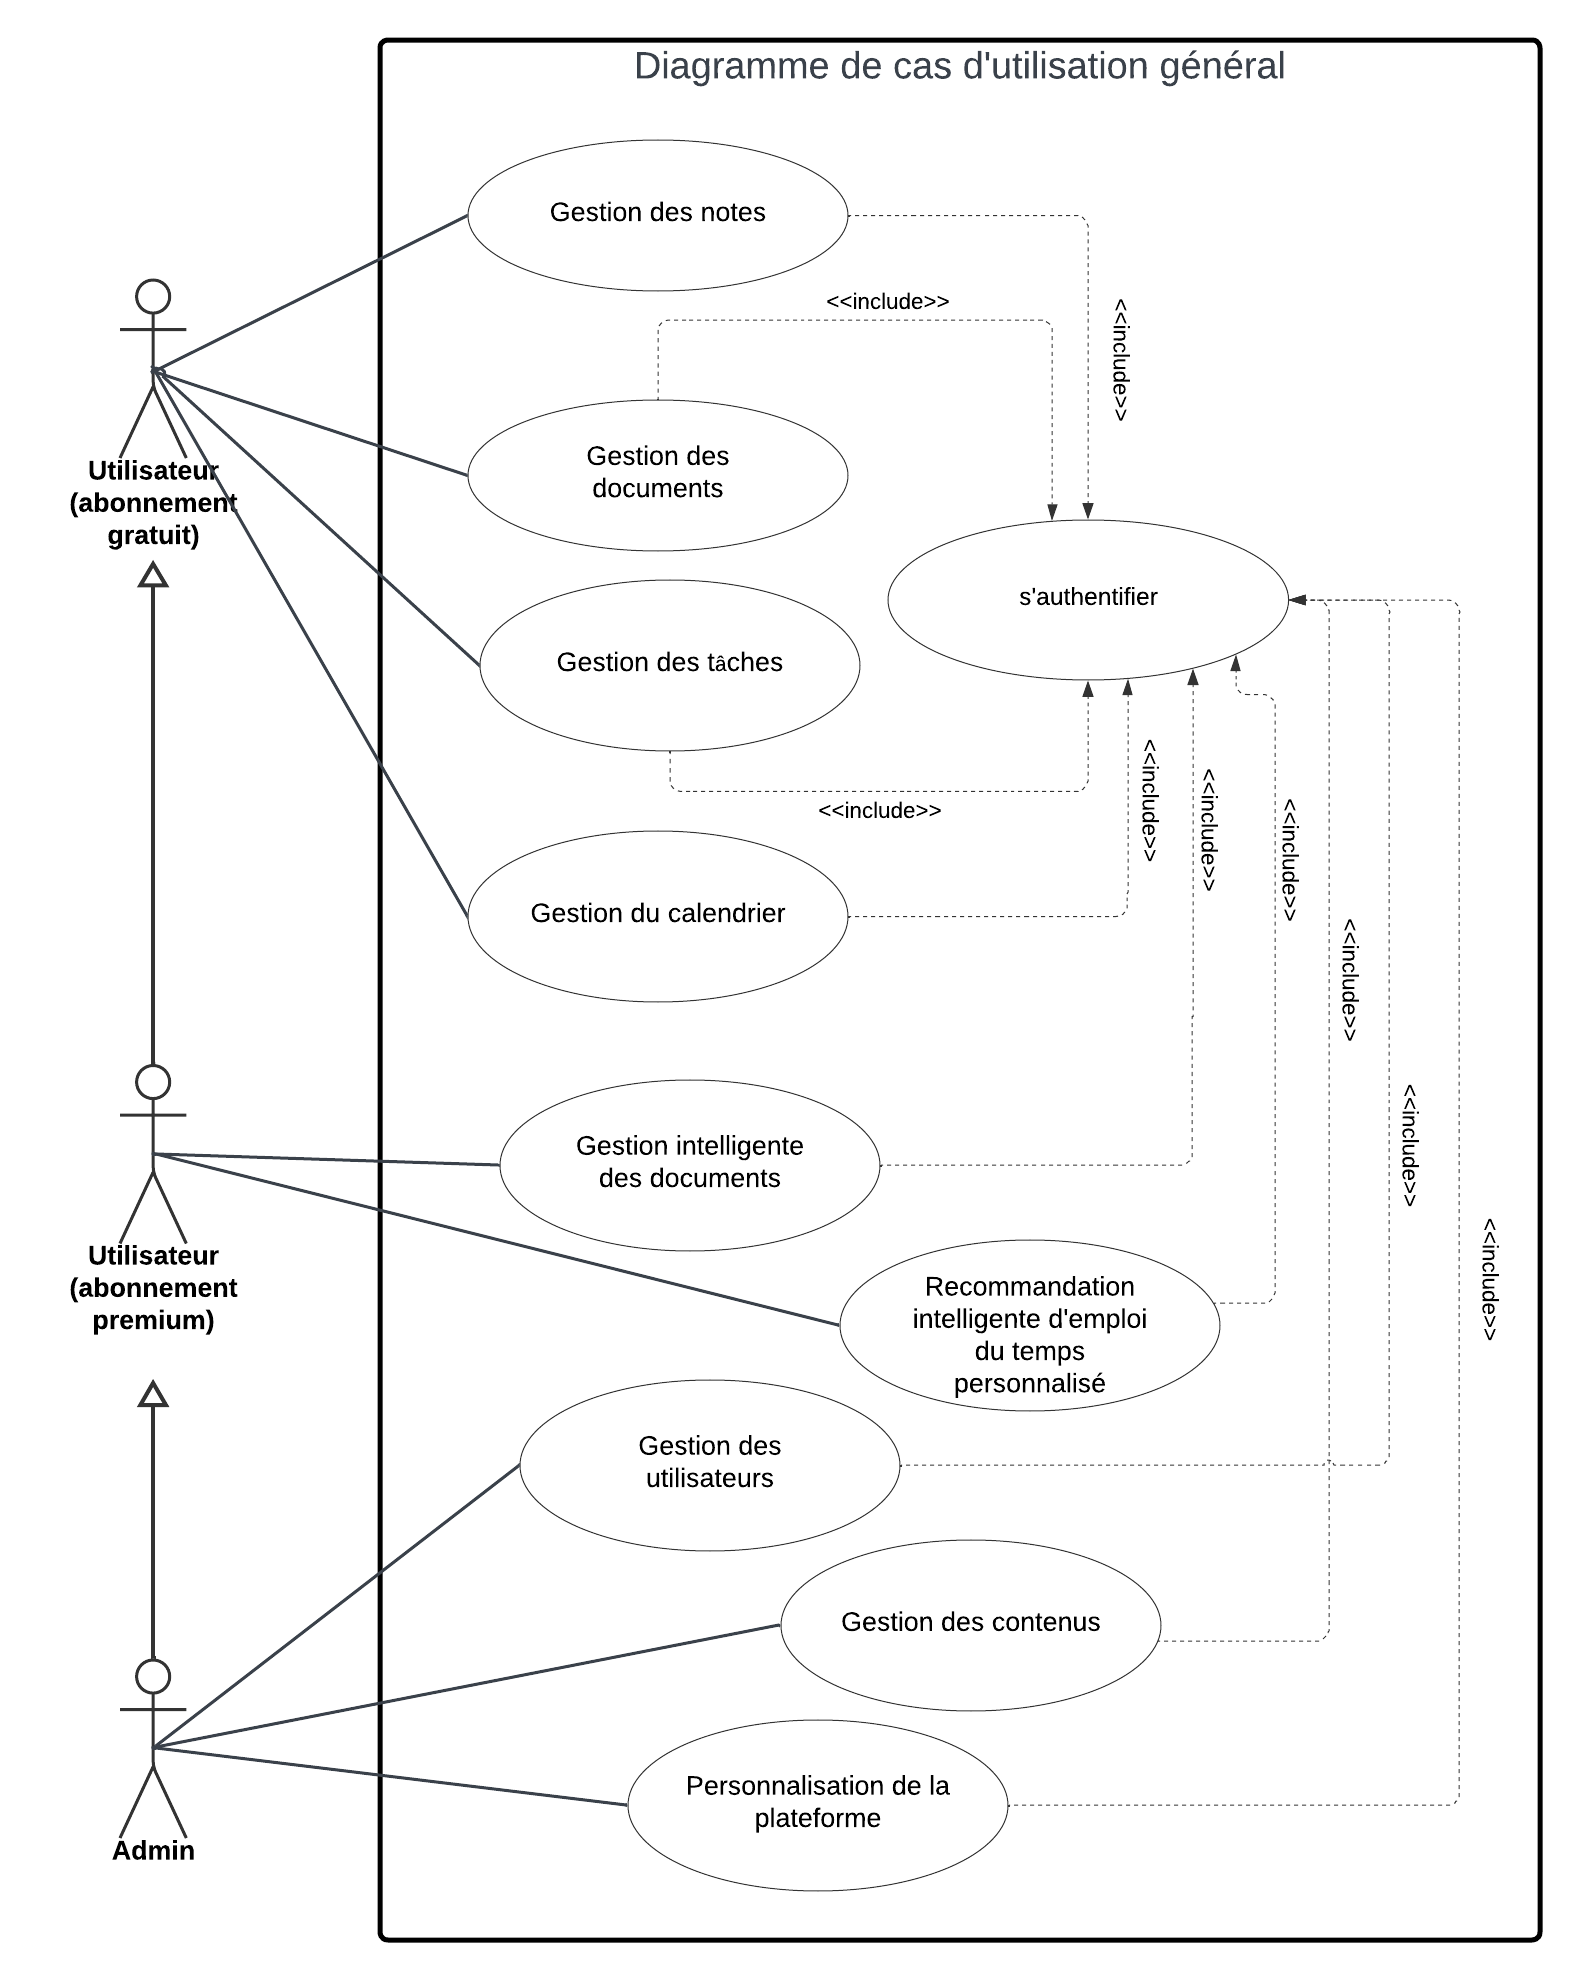
\includegraphics[scale=0.74]{chapitre2/figuresChap2/Use case ( GLOBAL ) (3).png}
  \caption{Diagramme de cas d’utilisation global }   
  \label{fig:usecase(global)}
\end{figure}
\vspace{5mm}

\subsection{Raffinement des cas d’utilisation}
\vspace{5mm}
Afin de mieux comprendre un fontionnement d'un cas d'utilisation, nous allons présenter une table descriptive pour les principaux cas d'utilisation.
\vspace{8mm}
\subsubsection{Analyse de cas d'utilisation : << Gestion des tâches >>}
\begin{figure}[H]
  \centering
  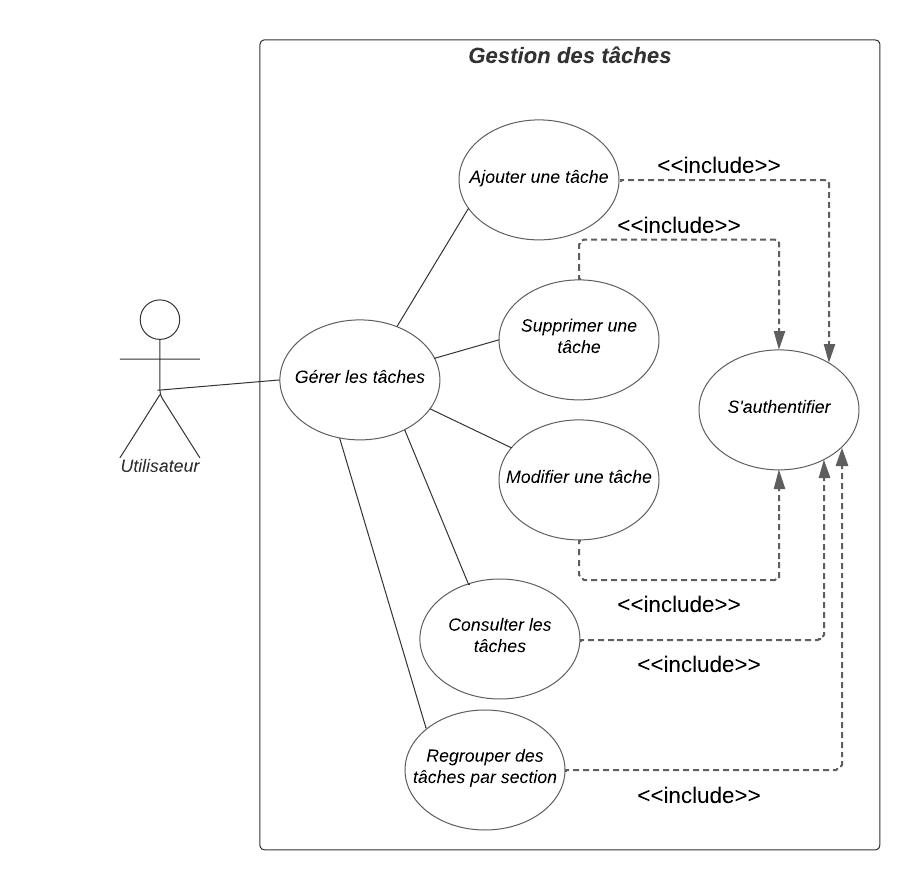
\includegraphics[scale=1.1]{chapitre2/figuresChap2/taches usecase 1.png}
  \caption{Diagramme de cas d’utilisation << Gestion des tâches >> }   
  \label{fig:usecase(taches)}
\end{figure}



Le tableau \ref{tab:gestion des tâches} indique la description textuelle du cas d'utilisation << Gestion des tâches >> :

\newpage
\begin{table}[htbp]
\caption{Description textuelle du cas d’utilisation <<Gestion des tâches>>}
    \begin{tabularx}{\textwidth}{|5|X|}
        \hline
        Cas d'utilisation & Gestion des tâches \\
        \hline
        Description & Ce cas d'utilisation décrit la gestion des tâches (ajouter, supprimer, modifier et consulter) \\
        \hline
        Acteurs & Tous \\
        \hline
        Post-condition & Une inerface affiche les tâches ajoutés. L'utilisateur peut consulter, supprimer ou modifier. \\
        \hline
        Scénario principal & \begin{itemize}[label=$\bullet$]
    \item Ajouter une tâche
    \item Parcourir les tâches
\end{itemize} En consultant les tâches, on peut:
\begin{itemize}[label=$\bullet$]
    \item Modifier les informations d'une tâche 
    \item Supprimer une tâche du section ou toute une section
    \item Marquer une tache comme terminée ou en attente
\end{itemize}
\\
        \hline
        Scénario alternatif & 
        \begin{itemize}[label=$\bullet$]
    \item Champs obligatoires non remplis
    \item Formats de données incorrects
\end{itemize}\\
        \hline
    \end{tabularx}
\label{tab:gestion des tâches}
\end{table}

\newpage

\subsubsection{Analyse de cas d'utilisation : << Gestion des notes >>}
\begin{figure}[H]
  \centering
  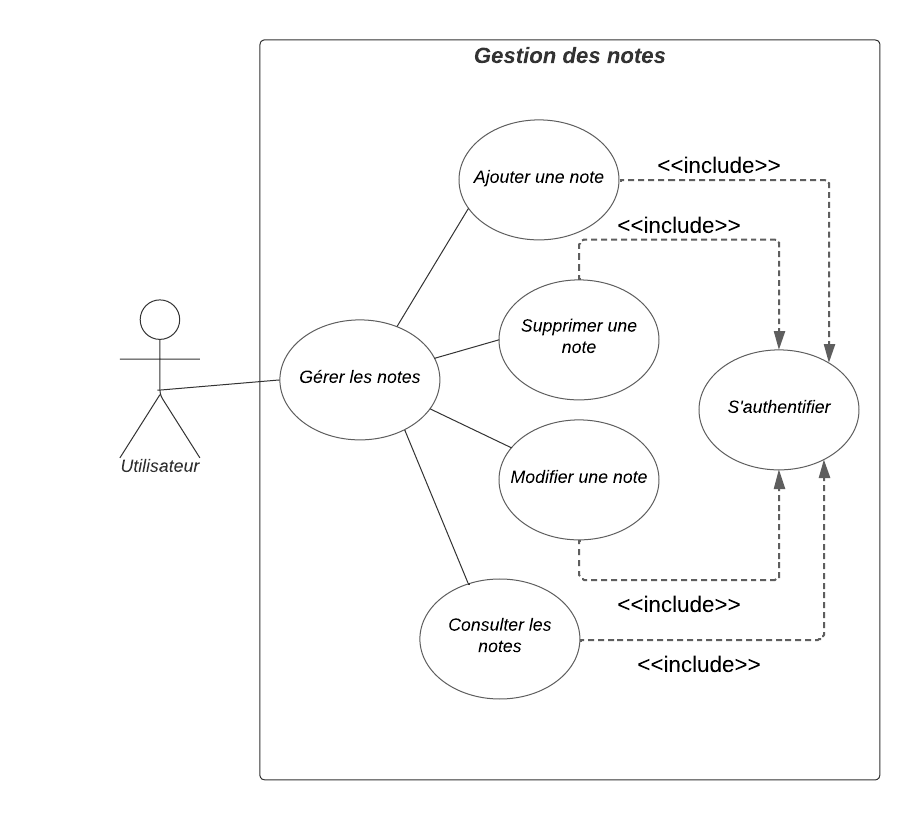
\includegraphics[scale=1.2]{chapitre2/figuresChap2/notes usecase 1.png}
  \caption{Diagramme de cas d’utilisation << Gestion des notes >> }   
  \label{fig:picture}
\end{figure}
Le tableau \ref{tab:gestion des notes} indique la description textuelle du cas d'utilisation << Gestion des notes >> :

\begin{table}[htbp]
\caption{Description textuelle du cas d’utilisation <<Gestion des notes>>}
    \begin{tabularx}{\textwidth}{|5|X|}
        \hline
        Cas d'utilisation & Gestion des notes \\
        \hline
        Description & Ce cas d'utilisation décrit la gestion des notes (ajouter, supprimer, modifier et consulter) \\
        \hline
        Acteurs & Tous \\
        \hline
        Post-condition & Une inerface affiche les notes ajoutés. L'utilisateur peut consulter, supprimer ou modifier. \\
        \hline
        Scénario principal & \begin{itemize}[label=$\bullet$]
    \item Ajouter une note
    \item Parcourir les notes
\end{itemize} En consultant les notes, on peut:
\begin{itemize}[label=$\bullet$]
    \item Modifier les informations d'une note 
    \item Supprimer une note
\end{itemize}
\\
        \hline
        Scénario alternatif & 
        \begin{itemize}[label=$\bullet$]
    \item Champs obligatoires non remplis
    \item Formats de données incorrects
    \item Format d'image non supporté
\end{itemize}\\
        \hline
    \end{tabularx}
\label{tab:gestion des notes}
\end{table}

\newpage

\subsubsection{Analyse de cas d'utilisation : << Gestion des documents >>}
\begin{figure}[H]
  \centering
  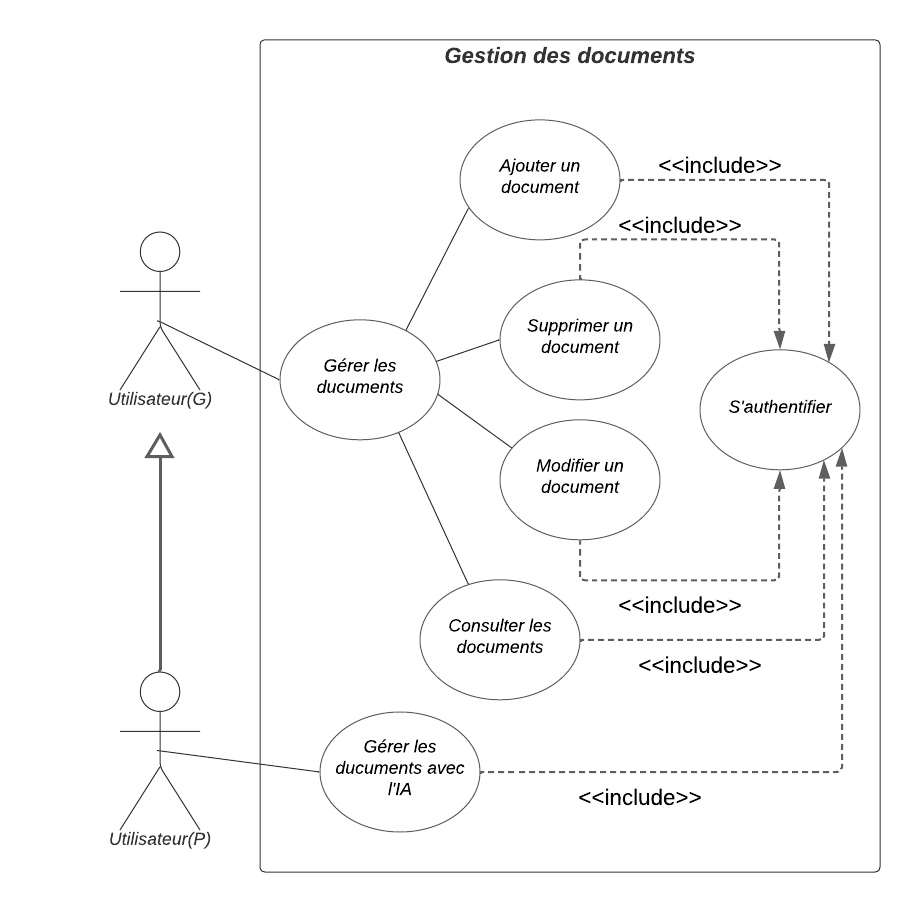
\includegraphics[scale=1]{chapitre2/figuresChap2/docmanager usecase (1).png}
  \caption{Diagramme de cas d’utilisation << Gestion des documents >> }   
  \label{fig:picture}
\end{figure}
Le tableau \ref{tab:gestion des documents} indique la description textuelle du cas d'utilisation << Gestion des documents >> :


\begin{table}[htbp]
\caption{Description textuelle du cas d’utilisation <<Gestion des notes>>}
    \begin{tabularx}{\textwidth}{|5|X|}
        \hline
        Cas d'utilisation & Gestion des documents \\
        \hline
        Description & Ce cas d'utilisation décrit la gestion des documents (ajouter, supprimer, modifier et consulter) \\
        \hline
        Acteurs & Tous \\
        \hline
        Post-condition & Une inerface affiche les documents regroupés dans des dossiers. L'utilisateur peut consulter, supprimer ou modifier. \\
        \hline
        Scénario principal & \begin{itemize}[label=$\bullet$]
    \item Ajouter un ou plusieurs documents
    \item AI analyse le document
    \item AI retourne le document dans son dossier de matière spécifique (ajouter un nouveau dossier si nécessaire)
\end{itemize} En consultant les documents, on peut:
\begin{itemize}[label=$\bullet$]
    \item Modifier le contenu d'un dossier 
    \item Supprimer un document ou un dossier
\end{itemize}
\\
        \hline
        Scénario alternatif & 
        \begin{itemize}[label=$\bullet$]
    \item Document est illisible ou corrompu.
    \item Classification incorrecte du document
    \item Format de document non supporté
    
\end{itemize}\\
        \hline
    \end{tabularx}
\label{tab:gestion des documents}
\end{table}



\newpage



\subsubsection{Analyse de cas d'utilisation : << Gestion du calendrier >>}
\begin{figure}[H]
  \centering
  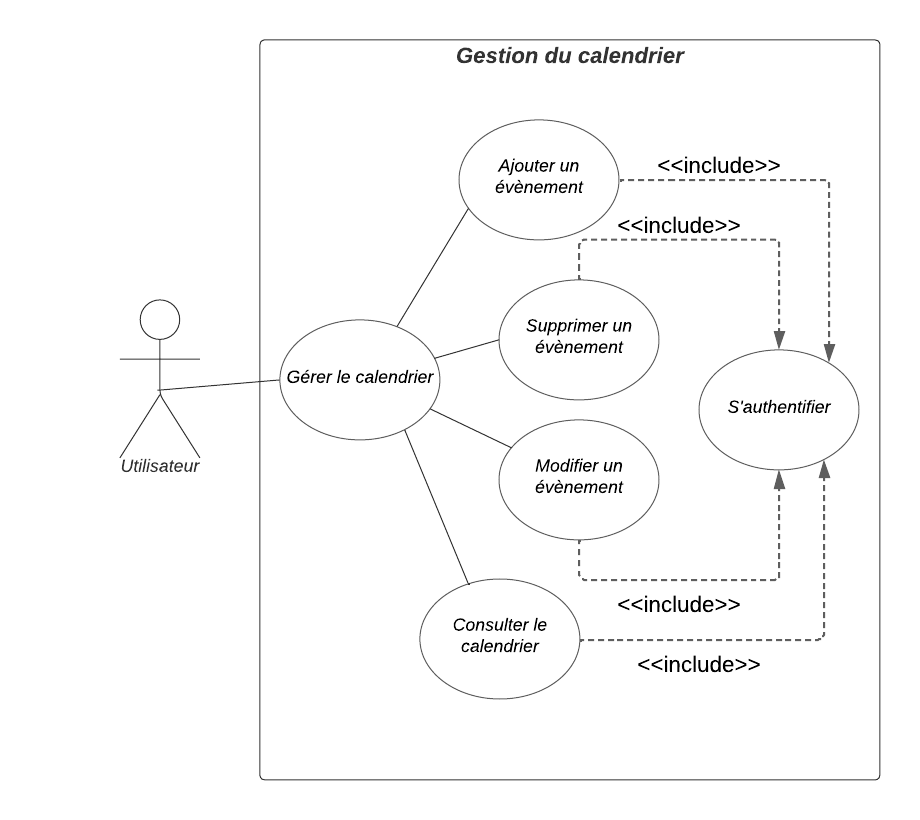
\includegraphics[scale=1.2]{chapitre2/figuresChap2/calander usecase 1.png}
  \caption{Diagramme de cas d’utilisation << Gestion du calendrier >> }   
  \label{fig:picture}
\end{figure}
Le tableau \ref{tab:gestion du calendrier} indique la description textuelle du cas d'utilisation << Gestion du calendrier >> :

\newpage

\begin{table}[htbp]
\caption{Description textuelle du cas d’utilisation <<Gestion du calendrier>>}
    \begin{tabularx}{\textwidth}{|5|X|}
        \hline
        Cas d'utilisation & Gestion du calendrier \\
        \hline
        Description & Ce cas d'utilisation décrit la gestion des évènements (ajouter, supprimer, modifier et consulter) \\
        \hline
        Acteurs & Tous \\
        \hline
        Post-condition & Une inerface affiche le calendrier (vue de mois,de semaine ou de jour).L'utilisateur peut consulter, supprimer ou modifier les évènements. \\
        \hline
        Scénario principal & \begin{itemize}[label=$\bullet$]
    \item Ajouter un évènement
    \item Parcourir le calendrier
\end{itemize} En consultant le calendrier, on peut:
\begin{itemize}[label=$\bullet$]
    \item Modifier les informations d'un évènement 
    \item Supprimer un évènement
\end{itemize}
\\
        \hline
        Scénario alternatif & 
        \begin{itemize}[label=$\bullet$]
    \item Conflits de planification lors de la modification ou l'ajout d'événements
\end{itemize}\\
        \hline
    \end{tabularx}
\label{tab:gestion du calendrier}
\end{table}








\section{Maquettes}
\vspace{5mm}
Placer les maquettes des interfaces dans ce chapitre, "Analyse et spécification des besoins", constitue une démarche stratégique visant à fournir une représentation concrète et détaillée de la manière dont l'application web répondra aux exigences identifiées lors de l'étude préliminaire du projet. \\Cette intégration permettra aux lecteurs de visualiser comment les besoins des utilisateurs seront traduits en fonctionnalités spécifiques, mettant en lumière la pertinence et l'efficacité de la solution proposée. \\ En présentant les maquettes à ce stade du rapport, nous offrons une transition naturelle entre la phase d'identification des besoins et celle de leur spécification, permettant ainsi une compréhension approfondie de la vision conceptuelle du projet et de sa concrétisation pratique.

\newpage

\subsection{Accueil}
\vspace{5mm}
L'interface d'accueil qui est illustrée par la figure  \ref{fig:accueil} comporte:
\vspace{3mm}
\begin{itemize}[label=$\bullet$]
    \item une vue globale sur les tâches de l'utilisateur ( les tâches complètes, en retard,\\ incomplètes etc.. ).
    \vspace{3mm}
    \item un graphe qui présente la progression hebdomadaire de l'utilisateur.
    \vspace{3mm}
    \item un graphe qui présente la distribution hebdomadaire des tâches de l'utilisateur.
\end{itemize}
\vspace{8mm}
\begin{figure}[H]
  \centering
  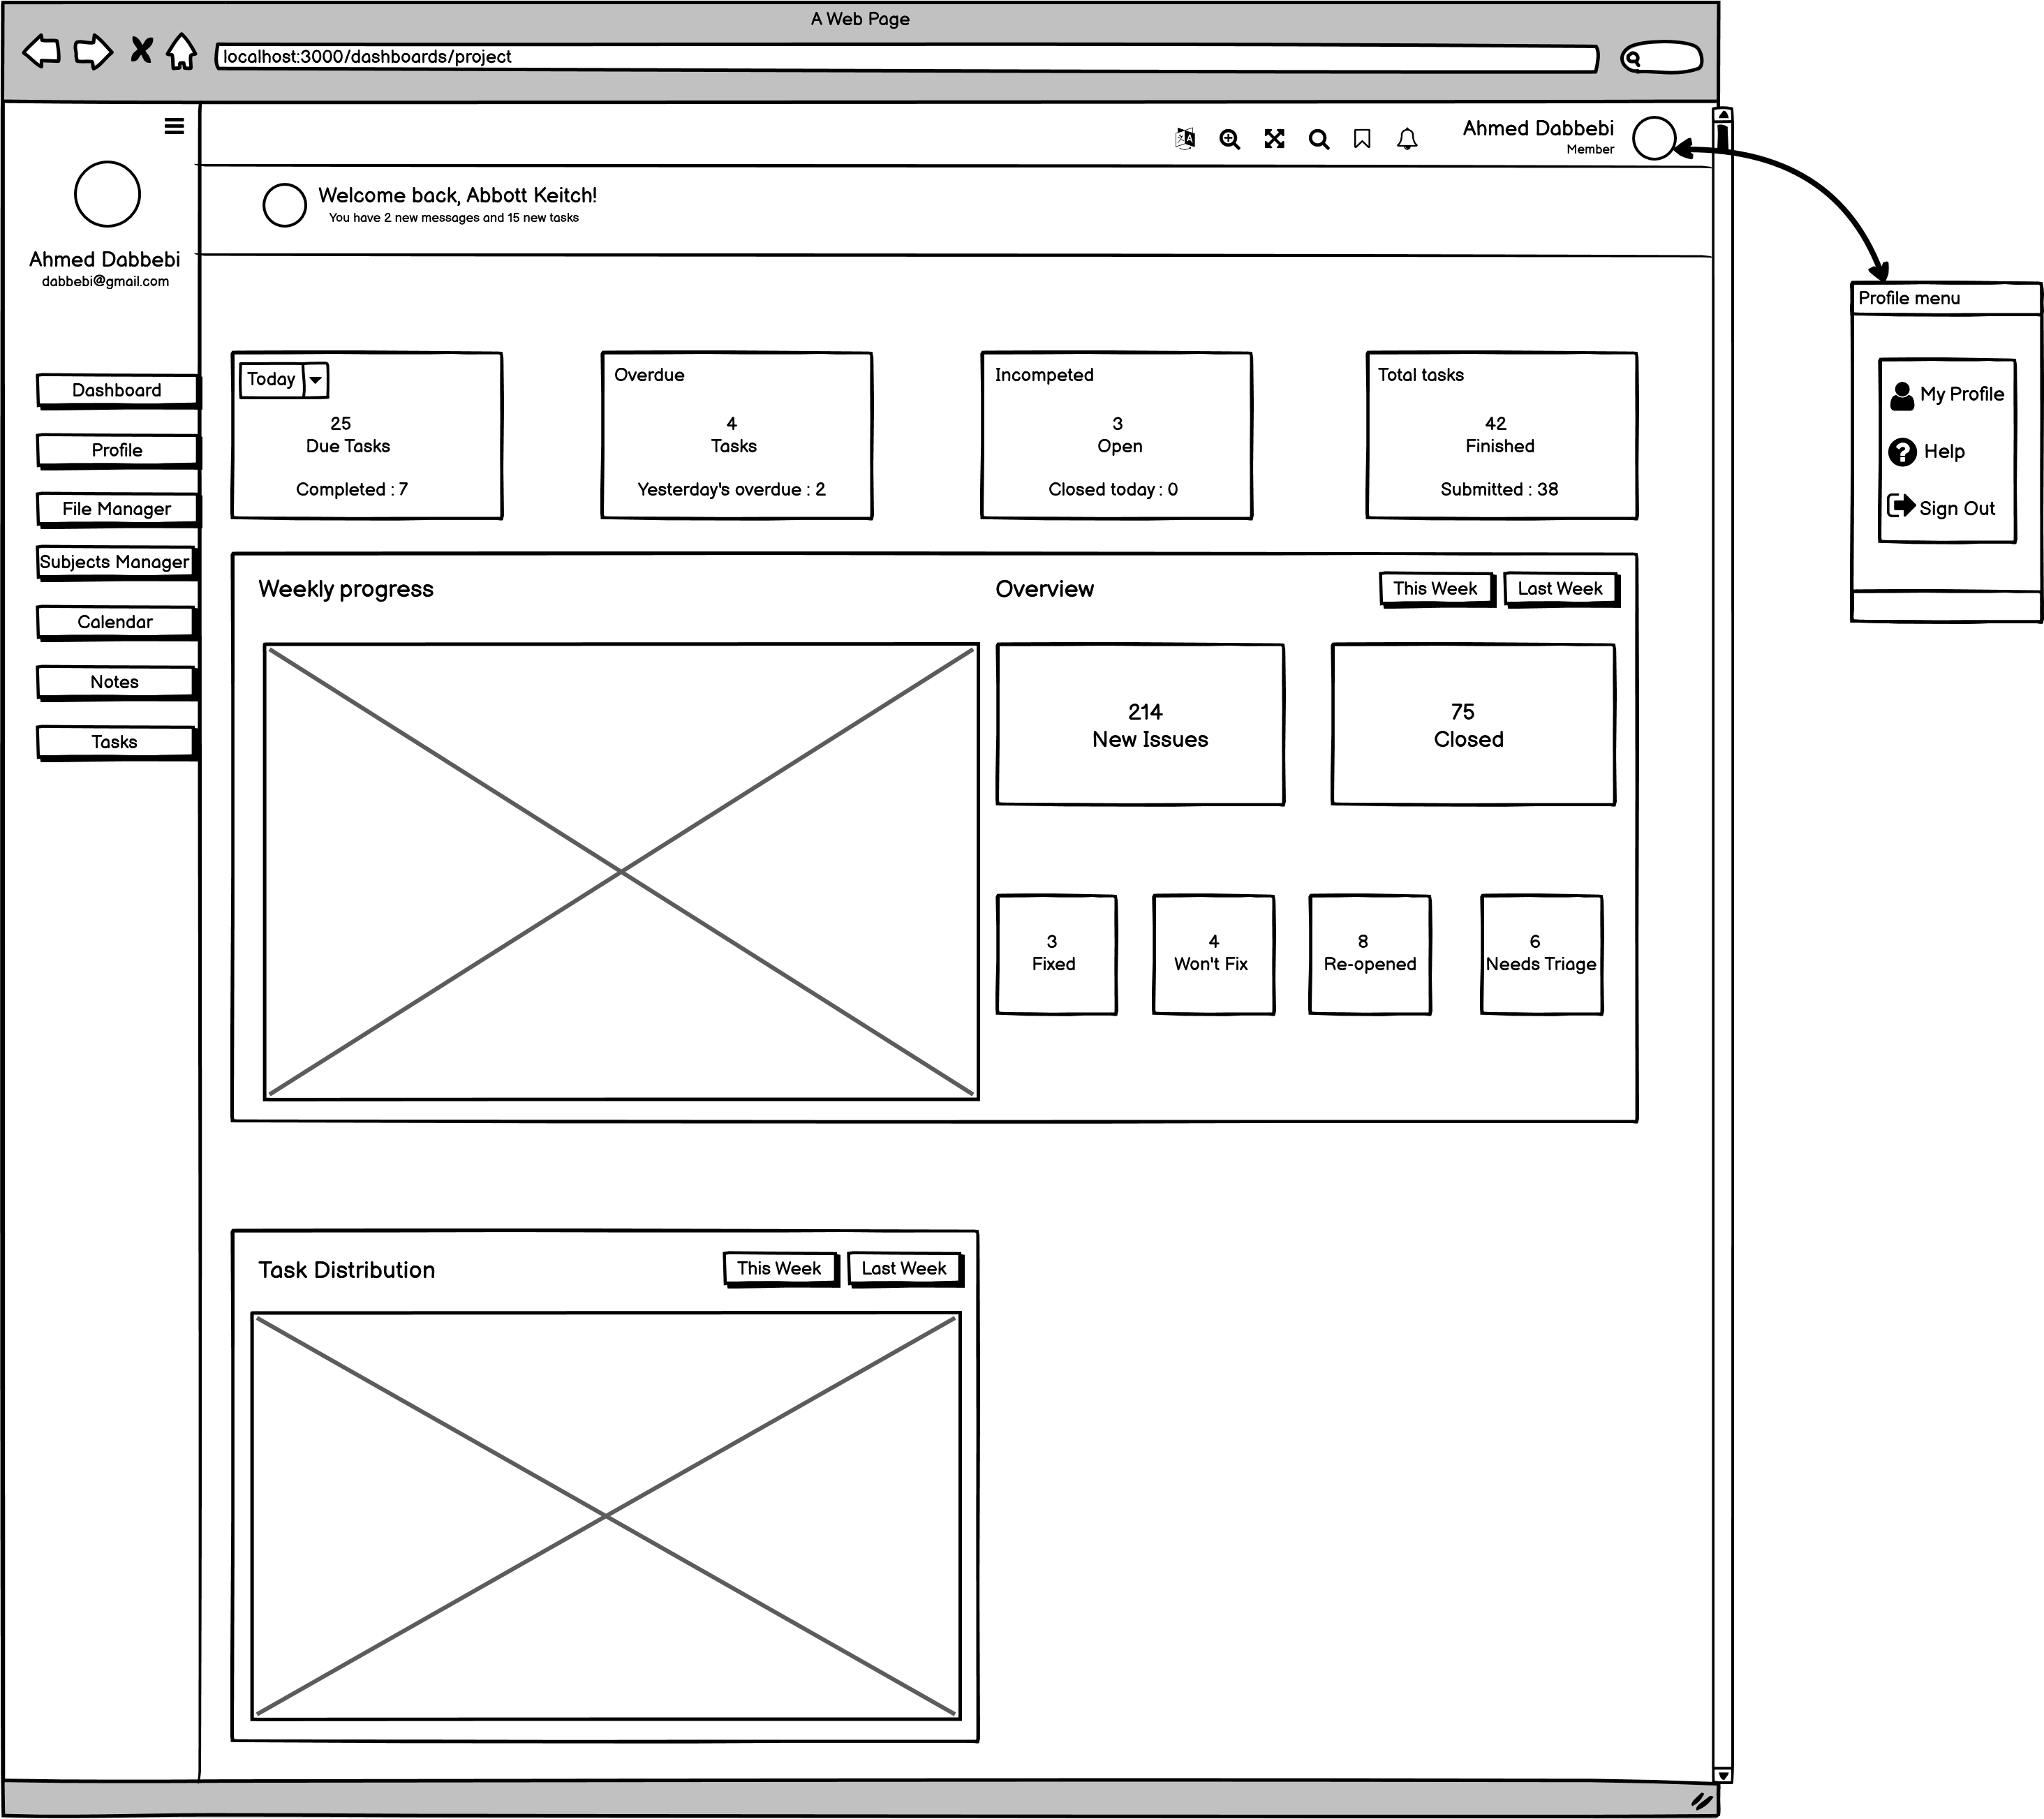
\includegraphics[scale=0.49]{chapitre2/maquettes/maquette/Dashboard(maquette).png}
  \caption{Interface de la page accueil}   
  \label{fig:accueil}
\end{figure}

\subsection{Gestionnaire des documents}
\vspace{5mm}
L'interface de gestionnaire des document qui est illustrée par la figure \ref{fig:documents} comporte:
\vspace{3mm}
\begin{itemize}[label=$\bullet$]
    \item une vue globale sur la classification des documents qui comporte:
    \vspace{3mm}
    \begin{itemize}[label=$\bullet$]
        \item une section qui regroupe les documents non classifiés.
        \vspace{3mm}
        \item une section qui regroupe les documents classifiés (dans des dossiers).
    \end{itemize}
    \vspace{3mm}
    \item une formulaire d'ajout d'un document en cliquant sur le bouton "Upload file"
\end{itemize}
\vspace{8mm}
\begin{figure}[H]
  \centering
  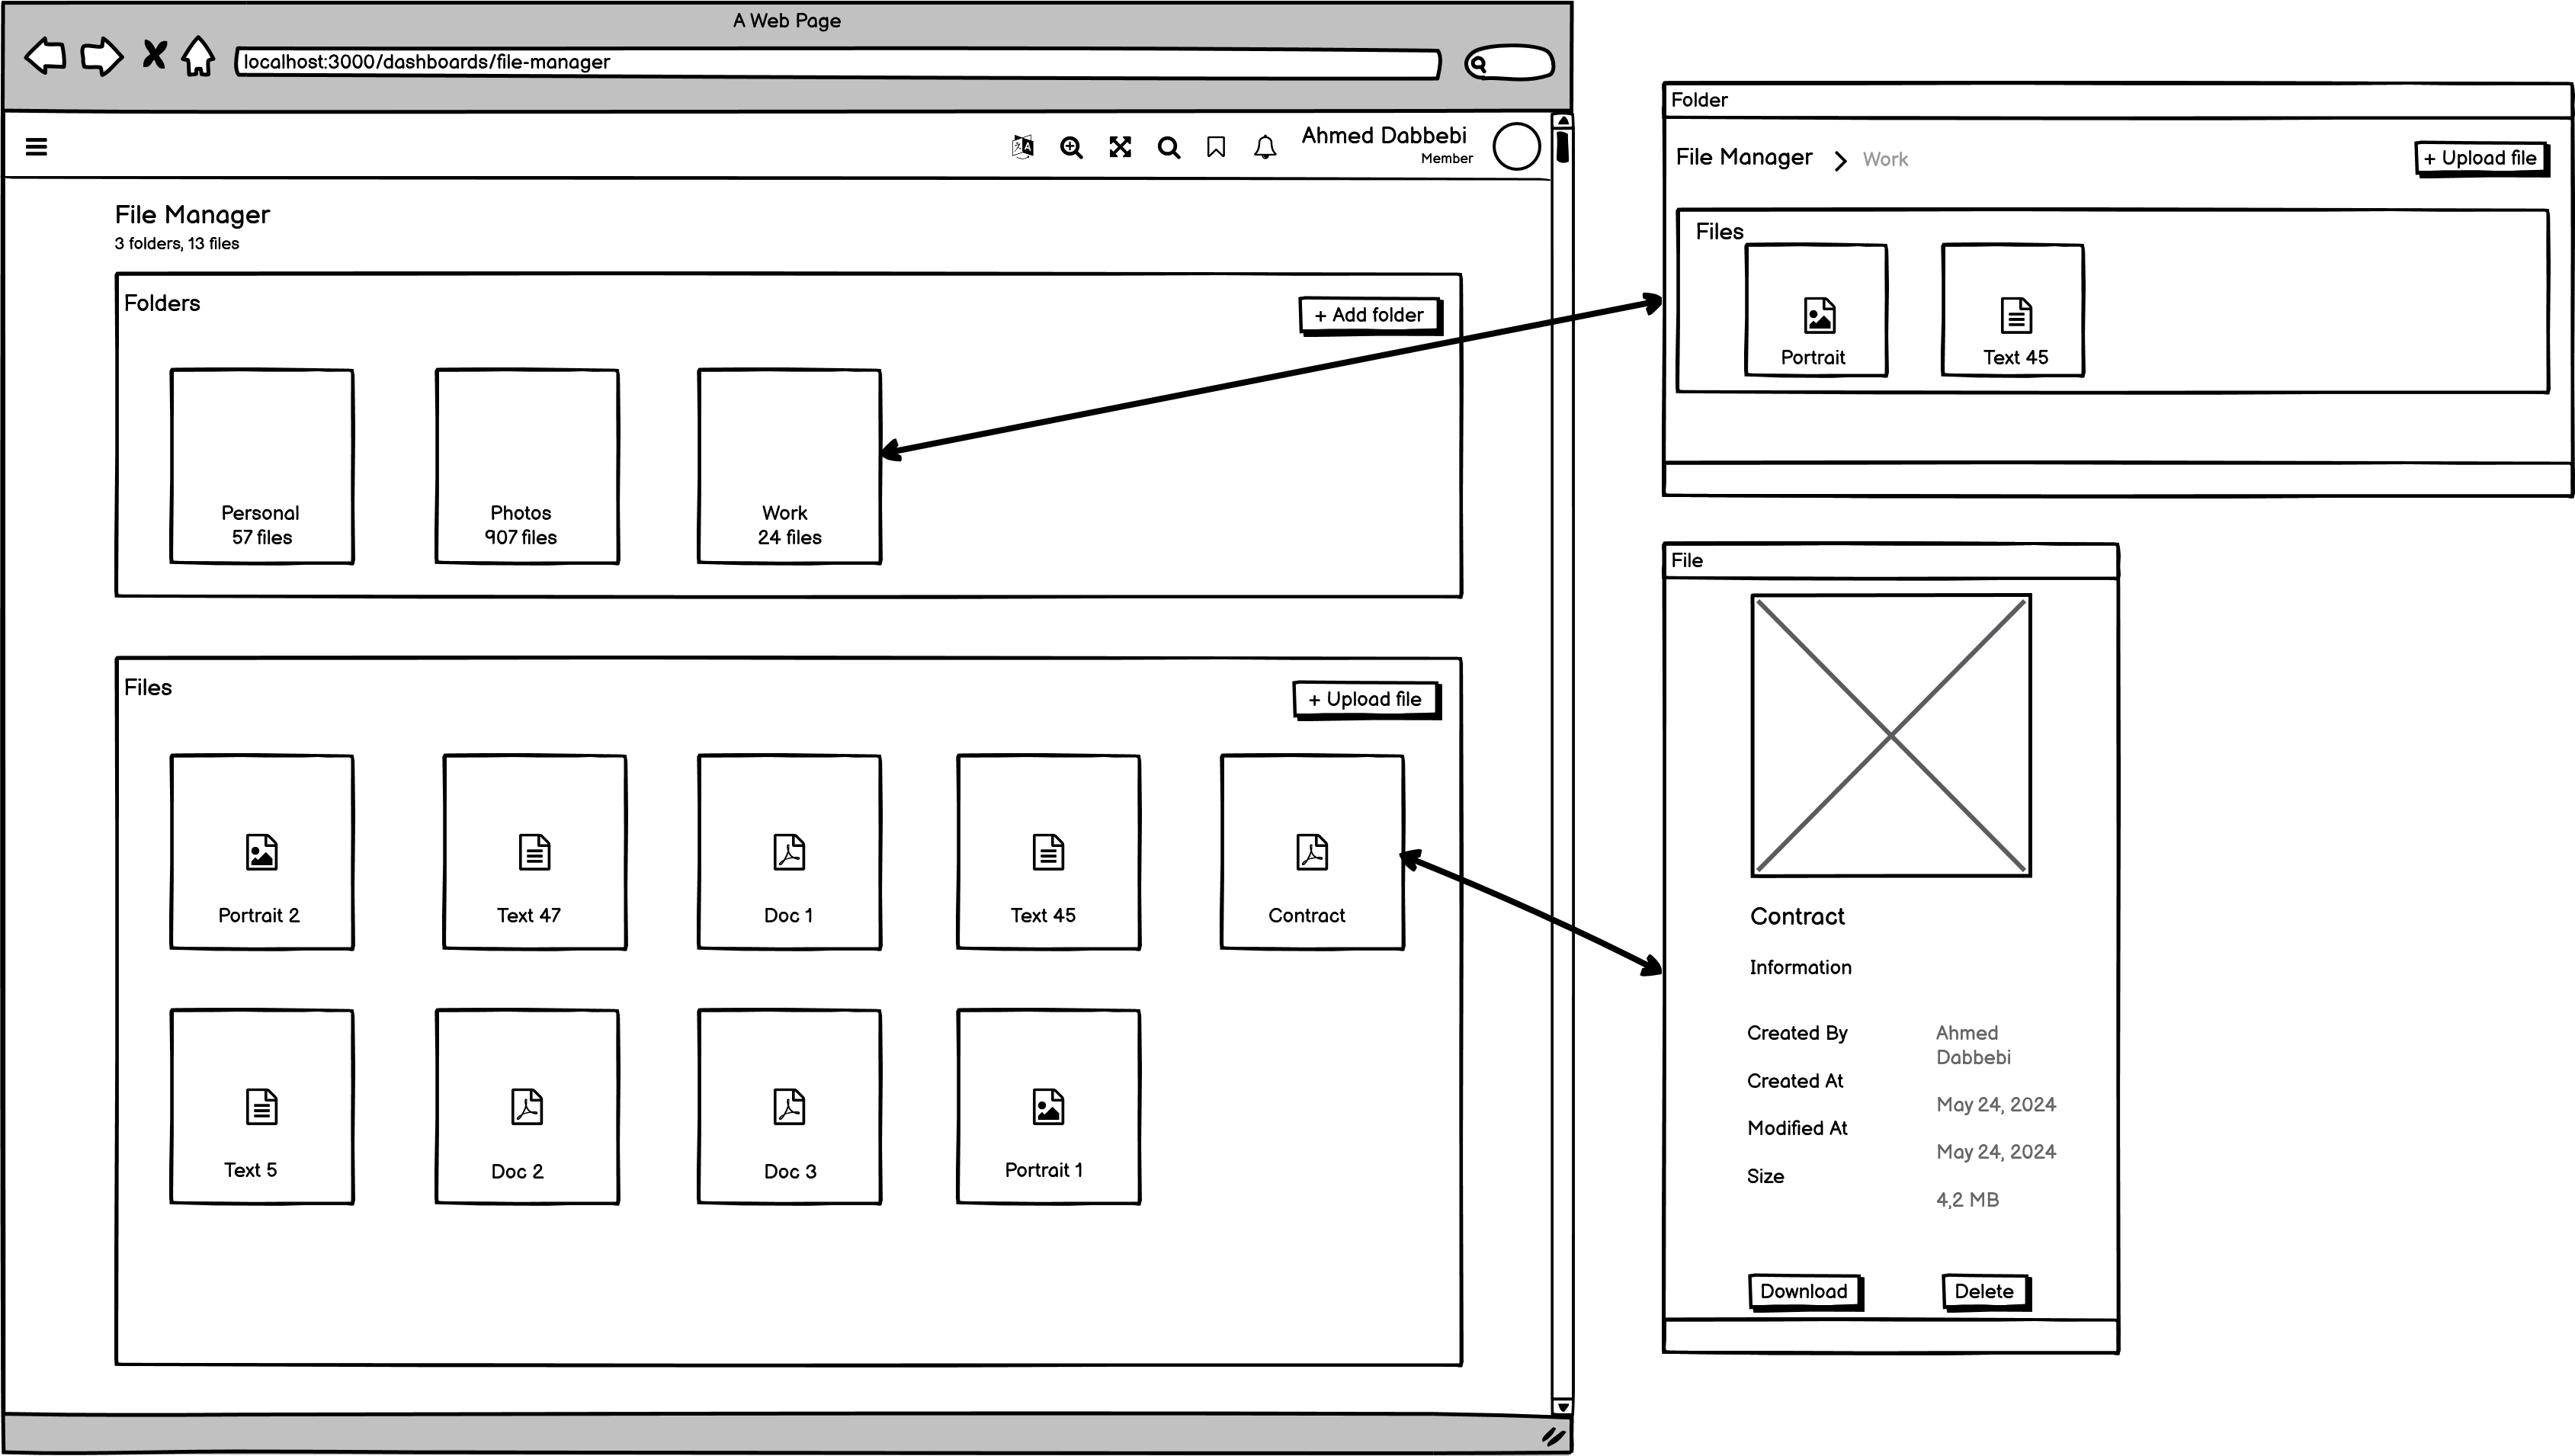
\includegraphics[scale=0.42]{chapitre2/maquettes/maquette/File Manager(maquette).png}
  \caption{Interface de la page gestionnaire des documents}   
  \label{fig:documents}
\end{figure}
\vspace{5mm}
\subsection{Calendrier}
\vspace{5mm}
L'interface de calendrier qui est illustrée par la figure \ref{fig:calendrier} comporte:
\vspace{3mm}
\begin{itemize}[label=$\bullet$]
    \item une vue globale (par mois, par semaine ou par jour) d'un calendrier qui comporte les évènements mis par l'utilisateur.
    \vspace{3mm}
    \item  une formulaire d'ajout d'un évènement en cliquant sur le bouton d'ajout.
    \vspace{3mm}
    \item un menu de modification de labels des évènements.
\end{itemize}
\vspace{4mm}
\begin{figure}[H]
  \centering
  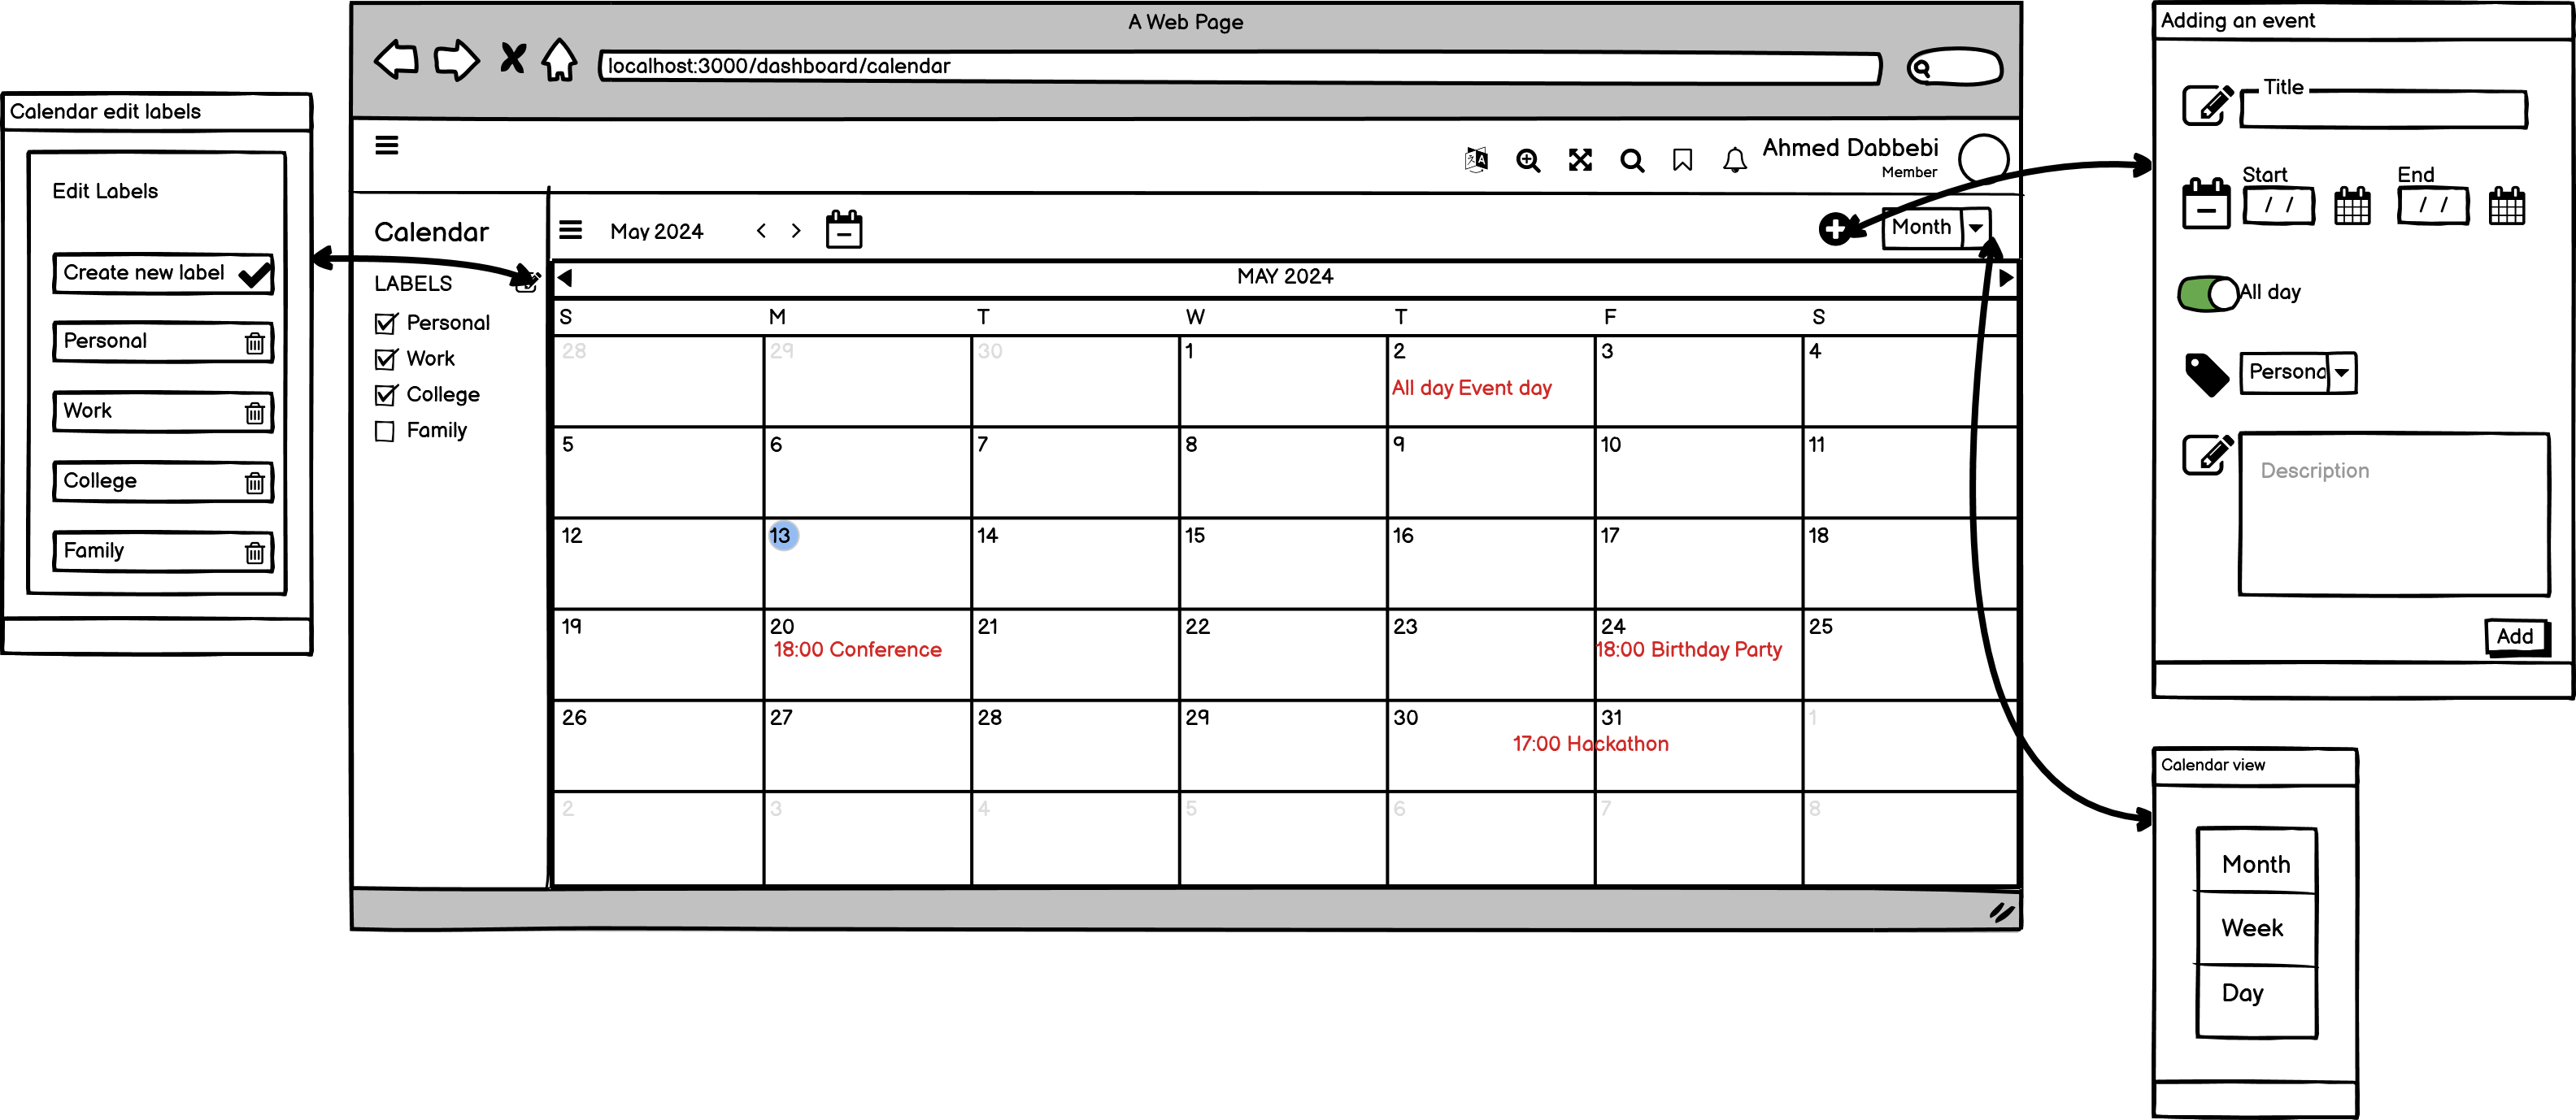
\includegraphics[scale=0.45]{chapitre2/maquettes/maquette/Calendar(maquette).png}
  \caption{Interface de la page calendrier}   
  \label{fig:calendrier}
\end{figure}
\vspace{5mm}
\subsection{Notes}
\vspace{5mm}
L'interface de notes qui est illustrée par la figure \ref{fig:notes} comporte:
\vspace{3mm}
\begin{itemize}[label=$\bullet$]
    \item une vue globale des notes crées par l'utilisateur.
    \vspace{3mm}
    \item une formulaire d'ajout d'une note en cliquant sur le champ de saisie de texte "Take a note".
    \vspace{3mm}
    \item un menu qui filtre les notes par ces labels, celles qui ont un rappel et celle qui ont été archivées.
    \vspace{3mm}
    \item un menu de modification de labels des notes.
\end{itemize}
\vspace{8mm}
\begin{figure}[H]
  \centering
  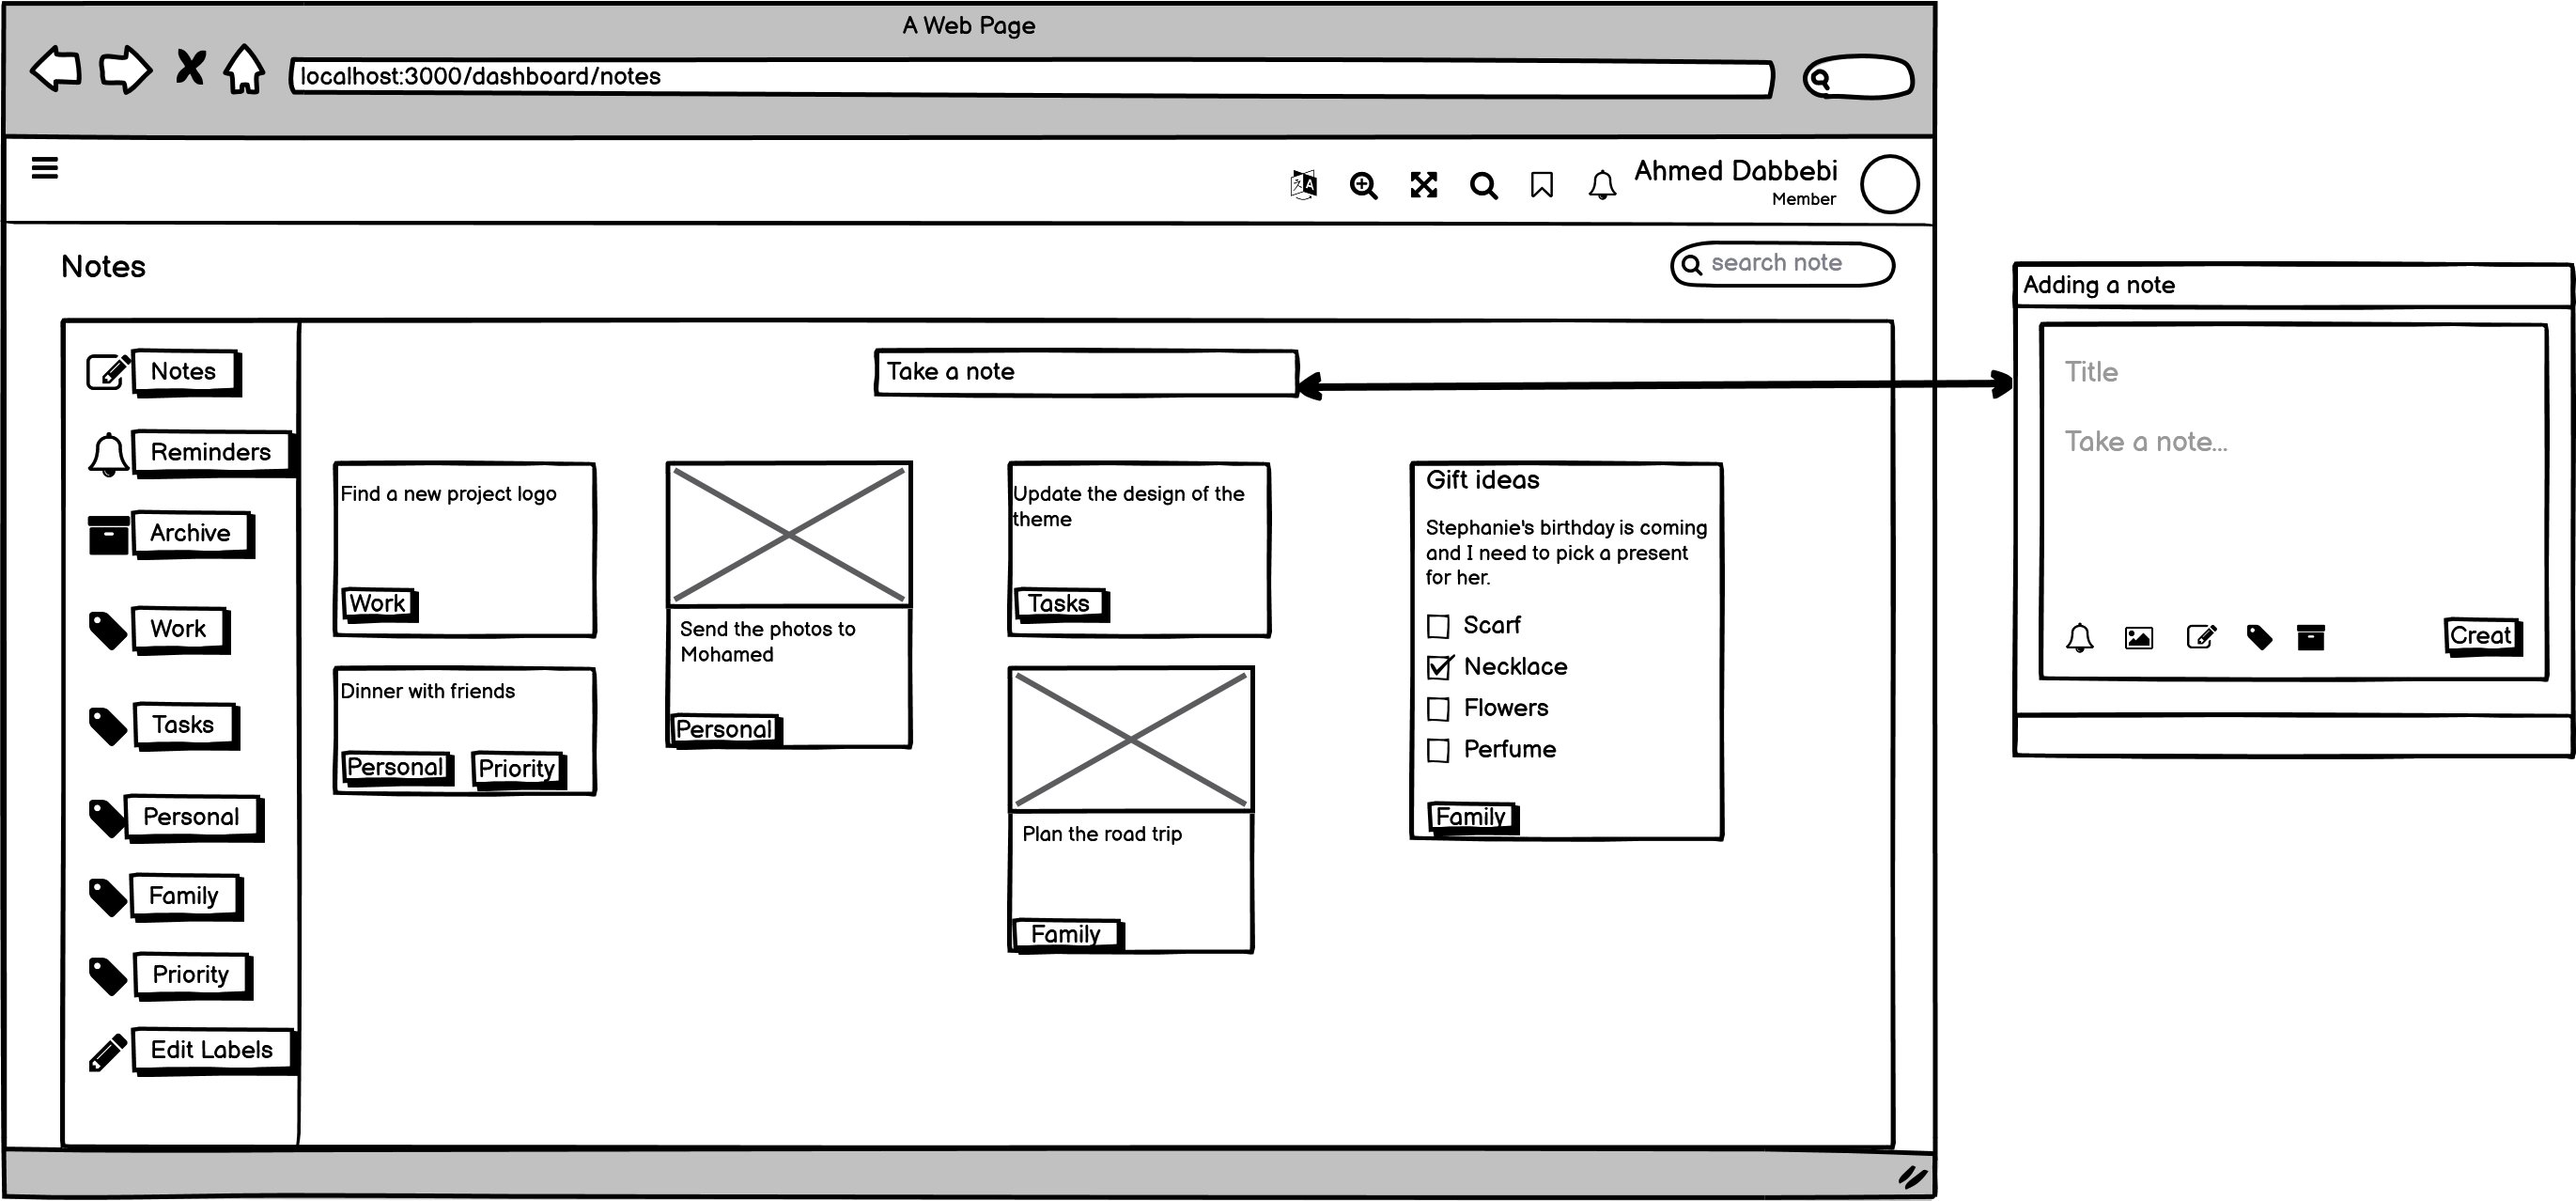
\includegraphics[scale=0.51]{chapitre2/maquettes/maquette/Notes(maquette).png}
  \caption{Interface de la page notes}   
  \label{fig:notes}
\end{figure}
\vspace{5mm}
\subsection{Tâches}
\vspace{5mm}
L'interface de tâches qui est illustrée par la figure \ref{fig:tâches} comporte:
\vspace{3mm}
\begin{itemize}[label=$\bullet$]
    \item une vue globale des tâches et sections crées par l'utilisateur.
    \vspace{3mm}
    \item une formulaire d'ajout d'une tâche en cliquant sur le bouton "Add Task".
    \vspace{3mm}
    \item une formulaire d'ajout d'une section en cliquant sur le bouton "Add Section".
\end{itemize}
\vspace{8mm}
\begin{figure}[H]
  \centering
  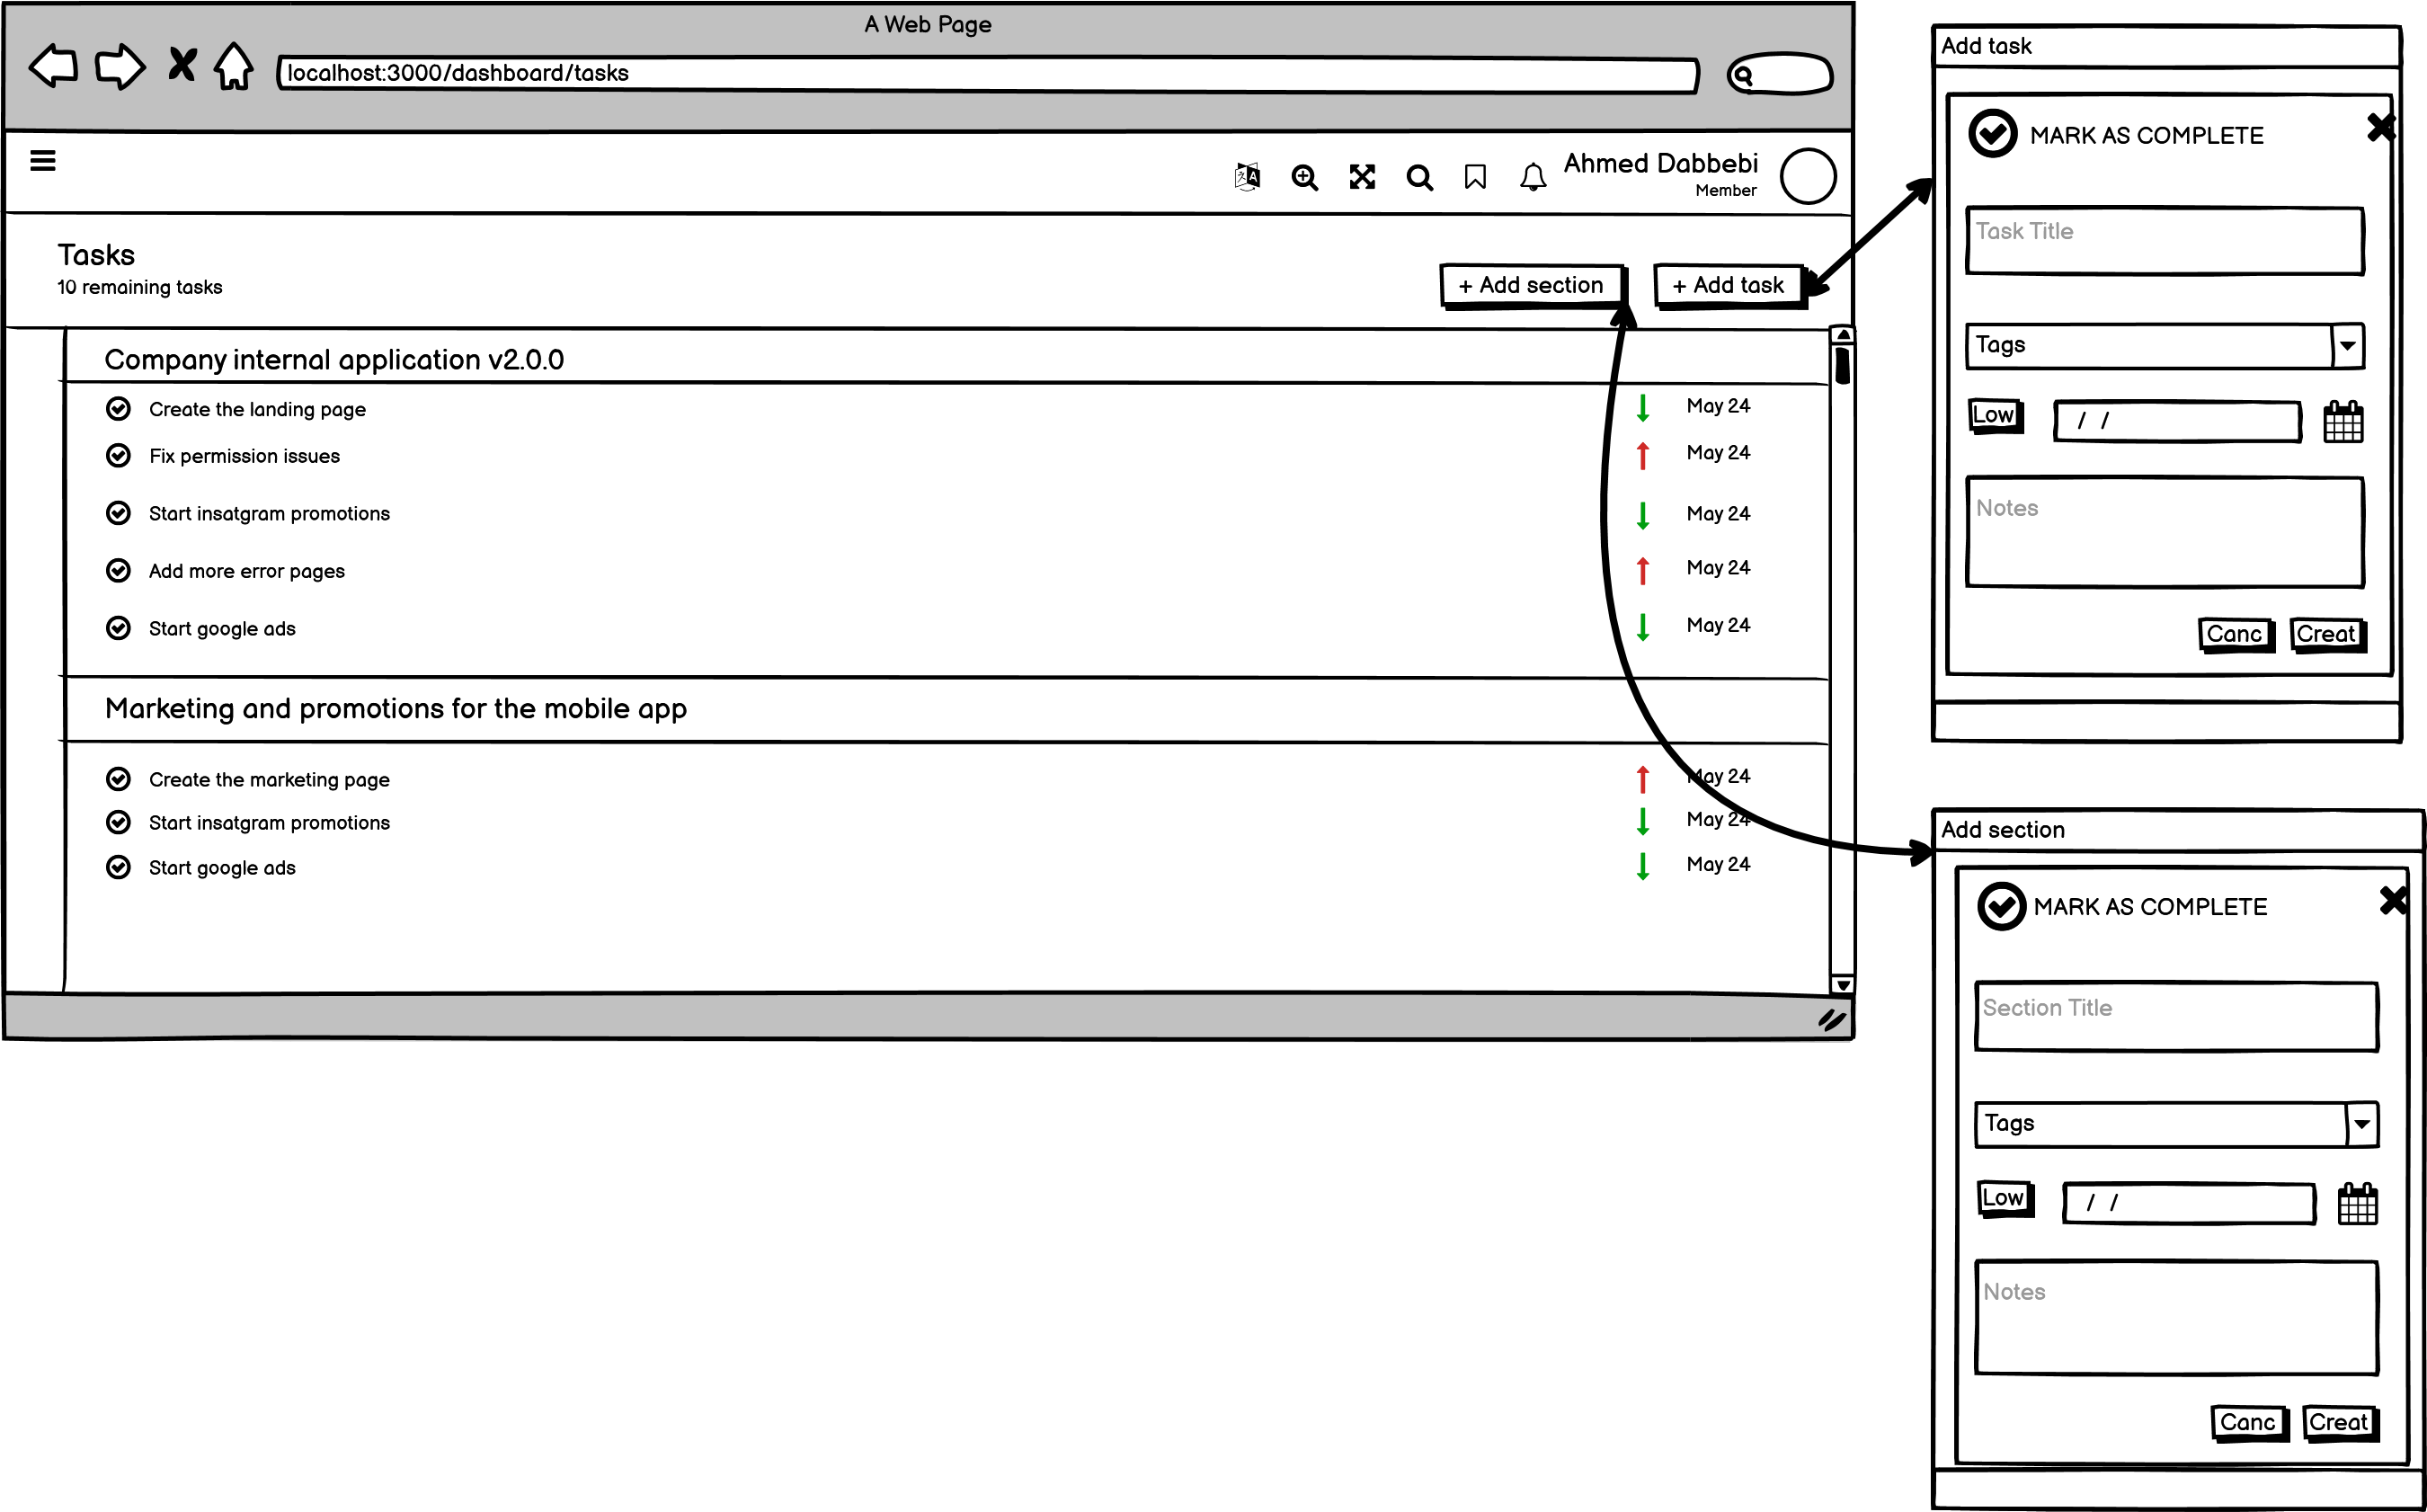
\includegraphics[scale=0.53]{chapitre2/maquettes/maquette/Tasks(maquettttte).png}
  \caption{Interface de la page tâches}   
  \label{fig:tâches}
\end{figure}



\section{Conclusion}
Au fil de ce chapitre, nous avons minutieusement analysé et spécifié les besoins fonctionnels et non-fonctionnels de notre projet, jetant ainsi les bases nécessaires à la réalisation de notre plateforme. Nous avons identifié les fonctionnalités essentielles ainsi que les exigences supplémentaires qui guideront le développement de la solution. Le prochain chapitre sera consacré à la conception.













